% !TeX encoding=utf8
% !TeX spellcheck = de_DE
% !TeX root = ../Diploma.tex

\chapter{Vergleich zwischen Kotlin und dem Google Web Toolkit}\label{sec:comparison}
Ziel dieses Kapitels soll der Vergleich von Kotlin und dem \gls{GWT} sein, da es im Zusammenhang mit der Programmiersprache Java auch zum Erstellen von Server-Client-Anwendungen geeignet ist.
Prinzipiell stellt \gls{GWT} einen Compiler bereit, mit welchem es möglich ist Java- nach JavaScript-Code zu kompilieren. Dabei ist aber zu beachten, dass Kotlin eine Programmiersprache und \gls{GWT} ein Framework ist, welches in und für Java implementiert wurde. Um einen sinnvollen Vergleich zu ermöglichen, wird im Nachfolgenden \gls{GWT} in Zusammenhang mit Java bzw. als Erweiterung betrachtet.\\
\\
In dem ersten \hyperref[sec:comparisonCriteria]{Unterabschnitt~\ref{sec:comparisonCriteria}} werden dafür zuallererst die Vergleichskriterien ermittelt, welche für den Vergleich benötigt werden. Anschließend dient der \hyperref[sec:comparisonResults]{Unterabschnitt~\ref{sec:comparisonResults}} zur Präsentation des Vergleichsergebnisses.\\
\\
Da für diese Arbeit die Benutzung der Programmiersprache Kotlin vorgegeben ist, wird auf eine Bewertung der Vergleichsteilnehmer verzichtet.

\section{Vergleichskriterien}\label{sec:comparisonCriteria}
Für die Ermittlung der Vergleichskriterien wurde das Paper \cite{frameworkEvaluation} von Jadhav und Sonar verwendet. In diesem werden zwar Bewertungsmethodiken für den Entscheidungsprozess von Software-Produkten ermittelt und näher erläutert, aber viele dieser Kriterien lassen sich auch auf Programmiersprachen anwenden. \\
\\
Jadhav und Sonar haben dafür, neben der Vorgehensweise eines Vergleichs, die sieben Hauptkriterien aus der \hyperref[fig:comparisionCriteria]{Abbildung~\ref{fig:comparisionCriteria}} entwickelt und anschließend diesen granularere Unterkriterien zugeordnet. Um eine Bewertung der einzelnen Kriterien zu vereinfachen, wurden diesen Leitfragen zugewiesen. Mit der Beantwortung dieser Fragen soll die Benotung vereinfacht werden.\\
\begin{figure}[htb]
	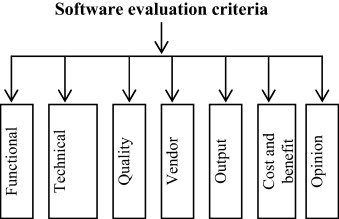
\includegraphics[width=0.5\textwidth]{images/comparision-criteria.jpg}
	\caption{Hauptkriterien des Softwarevergleichs von Jadhav und Sonar \cite{frameworkEvaluation}}
	\label{fig:comparisionCriteria}
\end{figure}
\\
Wie schon Anfangs erwähnt, lassen sich nicht alle Kriterien auf Programmiersprachen anwenden, weshalb für diesen konkreten Fall die Hauptkriterien \enquote{Technical} und \enquote{Output} entfallen. Da mit \enquote{Technical} Hardware- und mit \enquote{Output} Ausgabe-Kriterien gemeint sind, finden diese keine Verwendung.\\
\\
In den nachfolgenden \hyperref[sec:functionalCriteria, sec:opinionCriteria]{Unterabschnitten~\ref{sec:functionalCriteria} bis \ref{sec:opinionCriteria}} werden dafür den Hauptkriterien einzelne Unterkriterien zugeordnet und mit Leitfragen detaillierter beschrieben. Dabei beziehen sich diese auf den konkreten Anwendungsfall des Vergleichs, wobei die Kompilierung nach JavaScript im Vordergrund stehen soll.
%Auf Basis des Papers von Jadhav und Sonar wurden die Kriterien, aus der  \hyperref[tab:comparisonCriteria]{Tabelle~\ref{tab:comparisonCriteria}}, für diesen Anwendungsfall ausgearbeitet bzw. angepasst.
 
\subsection{Funktionale Kriterien (Functional)}\label{sec:functionalCriteria}
\subsubsection{JavaScript-Kompilierung}
\begin{itemize}
	\item In welche JavaScript-Versionen kann kompiliert werden?
	\item Welche Java-Script Modul-Systeme werden unterstützt?
\end{itemize}

\subsubsection{Build-Tools}
\begin{itemize}
	\item Welche Build-Tools werden offiziell unterstützt?
\end{itemize}

\subsubsection{Bibliotheken}
\begin{itemize}
	\item Können schon bestehende JavaScript-Bibliotheken eingebunden werden?
	\item Wie komfortabel ist die Einbindung bestehender Bibliotheken?
	\item Können Java-Bibliotheken eingebunden werden?
\end{itemize}

\subsubsection{Programmierung}
\begin{itemize}
	\item Welcher Programmierstil wird verwendet?
	\item Welcher Grad der Typisierung wird verwendet?
	\item Werden Aspekte der funktionalen Programmierung unterstützt?
%	\item Wie gut ist die Handhabung Funktionaler Aspekte sofern diese existieren?
\end{itemize}

\subsection{Qualitative Kriterien (Quality)}\label{sec:qualityCriteria}
\subsubsection{Kommunikationsstandards}
\begin{itemize}
	\item Welche gängigen Formate können standardmäßig verarbeitet werden?
	\item Können diese direkt in Objekte geparst werden?
\end{itemize}

\subsubsection{Browser-Support}
\begin{itemize}
	\item Welche Browser werden unterstützt?
\end{itemize}

\subsubsection{Lernkurve}
\begin{itemize}
	\item Wie leicht lässt sich die Programmiersprache erlernen bzw. bedienen?
	\item Gibt es Online-Plattformen, um die Programmiersprache auszuprobieren?
\end{itemize}
 
\subsection{Anwenderkriterien (Vendor)}\label{sec:vendorCriteria}
\subsubsection{Dokumentation}
\begin{itemize}
	\item Gibt es eine ausführliche Dokumentation?
	\item Gibt es offizielle Tutorials?
\end{itemize}

\subsubsection{Support}
\begin{itemize}
	\item Wird Support von Entwicklern angeboten?
	\item Gibt es ein offizielles Forum oder ähnliches?
	\item Auf welchen weiteren Community-Plattformen ist die Programmiersprache vertreten? 
\end{itemize}

\subsubsection{Community}
\begin{itemize}
	\item Wie viele Entwickler sind an der Programmierung der Sprache beteiligt?
	\item Gibt es Unternehmen, welche die Entwicklung unterstützen?
\end{itemize}

\subsection{Kosten- und Nutzenorientierte Kriterien (Cost and benefit)}\label{sec:costCriteria}
\subsubsection{Lizenz}
\begin{itemize}
	\item Wurde die Programmiersprache unter einer freien Lizenz veröffentlicht?
	\item Entstehen durch die Benutzung Lizenzkosten?
\end{itemize}

\subsubsection{Benutzungskosten}
\begin{itemize}
	\item Sind kostenpflichtige Programme für die Benutzung notwendig?
\end{itemize}

\subsection{Kriterien an die öffentliche Meinung (Opinion)}\label{sec:opinionCriteria}
\subsubsection{Beliebtheit}
\begin{itemize}
	\item Wie viele Repositories gibt es auf Github, welche mit der Programmiersprache entwickelt wurden?
	\item Wie viele Fragen wurden auf der Plattform Stack Overflow gestellt?
\end{itemize}

\subsubsection{Veröffentlichung}
\begin{itemize}
	\item Wann wurde die erste Version veröffentlicht?
\end{itemize}

\subsubsection{Indizes}
\begin{itemize}
	\item Welchen Platz hat die Programmiersprache beim Triobe Index belegt?
	\item Welchen Platz hat die Programmiersprache beim RedMonk Index belegt?
	\item Welchen Platz hat die Programmiersprache beim \gls{PYPL} Index belegt?
\end{itemize}
 
%{
%\small\renewcommand{\arraystretch}{1.4}
%\begin{longtabu} to \textwidth{X[1,L]X[1,L]X[2,L]}
%	\captionabove{Kriterien für den Vergleich zwischen Kotlin und dem Google Web Toolkit in Zusammenhang mit Java} \\
%	\hline
%	\taburowcolors 1{tableheadcolor .. tableheadcolor}
%	\bfseries Hauptkriterium &
%	\bfseries Unterkriterium &
%	\bfseries Leitfragen \\ \hline
%	\endfirsthead
%	\hline
%	Hauptkriterium &
%	Unterkriterium &
%	Leitfragen \\ \hline
%	\endhead
%	\hline
%	\taburowcolors 1{white .. white}
%	\multicolumn{3}{r}{\emph{weiter auf der nächsten Seite \ldots}}
%	\endfoot
%	\hline
%	\endlastfoot
%	\taburowcolors 2{tablebodycolor .. tablerowcolor}
%	Funktional (Functional) 
%		& JavaScript-Kompilierung 
%			& In welche JavaScript-Versionen kann kompiliert werden? \\
%			&& Welche JavaScript Modul-Systeme werden unterstützt? \\
%		& Build-Tools 
%			& Welche Build-Tools werden offiziell unterstützt? \\
%		& Bibliotheken 
%			& Können schon bestehende JavaScript Bibliotheken eingebunden werden? \\
%			&& Wie komfortable ist die Einbindung bestehender Bibliotheken? \\
%			&& Können Java-Bibliotheken eingebunden werden? \\
%		& Programmierung 
%			& Welcher Programmierstil wird verwendet? \\
%			&& Welcher Grad der Typisierung wird verwendet? \\
%			&& Werden Aspekte der Funktionalen Programmierung unterstützt? \\
%			&& Wie gut ist die Handhabung Funktionaler Aspekte sofern diese existieren? \\
%	Qualität (Quality) 
%		& Kommunikationsstandards 
%			& Welche gängigen Formate können standardmäßig verarbeitet werden? \\
%			&& Können diese direkt in Objekte geparst werden? \\
%		& Browser-Support
%			& Welche Browser werden unterstützt? \\
%		& Lernkurve 
%			& Wie leicht lässt sich die Programmiersprache erlernen bzw. bedienen? \\
%			&& Gibt es Online-Plattformen um die Programmiersprache auszuprobieren? \\
%	Anbieter (Vendor) 
%		& Dokumentation 
%			& Gibt es eine ausführliche Dokumentation? \\
%			&& Gibt es offizielle Tutorials? \\
%		& Support
%			& Wird Support von Entwicklern angeboten? \\
%			&& Gibt es ein offizielles Forum oder ähnliches? \\
%			&& Auf welchen weiteren Community-Plattformen ist die Programmiersprache vertreten? \\
%		& Community
%			& Wie viele Entwickler sind an der Programmiersprache beteiligt? \\
%			&& Gibt es Unternehmen welche die Entwicklung unterstützen? \\
%	Kosten und Nutzen (Cost and benefit) 
%		& Lizenz 
%			& Wurde die Programmiersprache unter einer freien Lizenz veröffentlicht? \\
%			&& Entstehen bei der Benutzung Lizenzkosten? \\
%		& Benutzungskosten
%			& Sind kostenpflichtige Programme für die Benutzung notwendig? \\
%	Meinungen (Opinion) 
%		& Beliebtheit 
%			& Wie viele Repositories gibt es auf Github, welche mit der Programmiersprache entwickelt wurden? \\
%			&& Wie viele Fragen wurden auf der Plattform Stackoverflow zu dieser Programmiersprache gestellt? \\
%		& Veröffentlichung
%			& Wann wurde die erste Version veröffentlicht? \\
%		& Tiobe Index
%			& Welchen Platz hat die Programmiersprache belegt? \\
%		& RedMonk Index
%			& Welchen Platz hat die Programmiersprache belegt? \\
%		& PYPL
%			& Welchen Platz hat die Programmiersprache belegt? \\
%\end{longtabu}
%}\label{tab:comparisonCriteria}

\section{Vergleichsergebnis}\label{sec:comparisonResults}

\subsection{Funktionale Kriterien (Functional)}
\subsubsection{JavaScript-Kompilierung}
\begin{description}
	\item[Kotlin] Als Ziel der Kompilierung dient der JavaScript-Standard ECMAScript 5. Es existieren aber bereits Pläne für die Umsetzung des ECMAScript 2015 Standards. Als Modul-System kann zwischen \gls{AMD}, CommonJS und \gls{UMD} gewählt werden. \cite{kotlinJavaScript, kotlinJsModules} 
	\item[GWT(Java)] Der Standard ECMAScript 5 dient auch für \gls{GWT} als Kompilierungsziel. Aber auch hier ist bereits eine Planung für den ECMAScript 2015 Standard bekannt, welcher mit der Version 3.0 veröffentlicht werden soll. Eine Verwendung eines JavaScript-Modul-Systems ist derzeit mit \gls{GWT} nicht möglich. \cite{gwtRoadmap}
\end{description}

\subsubsection{Build-Tools}
\begin{description}
	\item[Kotlin] Es werden gleich eine ganze Reihe an Build-Tools unterstützt. Vertreten sind dabei Gradle, Maven und Ant. Dabei wird aber die Nutzung von Gradle für die Kompilierung nach JavaScript offiziell empfohlen. \cite{kotlinBuildTools, kotlinToJavaScript}
	\item[GWT(Java)] Nur Ant wird unterstützt bzw. gibt es nur zu diesem eine offizielle Dokumentation. Aber dennoch können auch andere Build-Tools wie zum Beispiel Maven oder Gradle über Drittanbieter-Software verwendet werden. \cite{gwtGettingStarted}
\end{description}

\subsubsection{Bibliotheken}
\begin{description}
	\item[Kotlin] Es besteht die Möglichkeit bereits erstellte JavaScript-Bibliotheken, mittels \gls{JsInterop} zu integrieren. Dafür muss die \gls{API} der Bibliothek nachgebaut werden. Da das für große Projekte sehr mühselig sein kann, bietet Kotlin dafür das Tool \enquote{ts2kt}\footnote{siehe \url{https://github.com/Kotlin/ts2kt}} an, welches diese Aufgabe übernimmt. Voraussetzung dafür ist nur die Existenz der zugehörigen TypeScript Definitionsdateien. Eine Integration von Java-Bibliotheken ist nicht möglich. \cite{kotlinJsInteop, kotlinJsJavaToJs}
	\item[GWT(Java)] Ebenso wie in Kotlin besteht die Möglichkeit der Einbindung bereits bestehender JavaScript-Bibliotheken mithilfe von \gls{JsInterop} oder den \gls{JSNI}. Es wird jedoch nicht mehr empfohlen  \gls{JSNI} zu benutzen, weil diese Technologie veraltet ist und außerdem mit der dritten Version entfernt wird. Im Gegensatz zu Kotlin können in \gls{GWT} auch Java-Bibliotheken eingebunden werden. Was daher kommt, dass \gls{GWT} generell Java- in JavaScript-Code kompiliert. \cite{gwtJsInterop, gwtJSNI}
\end{description}

\subsubsection{Programmierung}
\begin{description}
	\item[Kotlin] Kotlin ist eine statisch typisierte und objekt-orientierte Programmiersprache, welche aber ebenso Aspekte der Funktionalen Programmierung enthält. \cite{kotlinInfo}
	\item[GWT(Java)] Auch wie Kotlin ist Java eine statisch typisierte und objekt-orientierte Programmiersprache. Funktionale Aspekte wie Lambda-Ausdrücke sind seit der Version acht verfügbar. \cite{java8Specification}
\end{description}

\subsection{Qualitative Kriterien (Quality)}
\subsubsection{Kommunikationsstandards}
\begin{description}
	\item[Kotlin] Mithilfe der Bibliothek \enquote{kotlinx.serialization} können die Formate \gls{JSON}, \gls{CBOR} und \gls{Protobuf} verarbeitet und auch direkt in Objekte geparst werden.
	Dabei besteht auch die Möglichkeit, die Bibliothek für andere Formate zu erweitern. Das Format \gls{XML} kann auch mit Standard JavaScript Methoden verarbeitet, aber nicht direkt in Objekte geparst werden. \cite{kotlinxSerialization}
	\item[GWT(Java)] Auch \gls{GWT} bietet die Möglichkeit \gls{JSON} direkt in Objekte zu parsen, aber genau wie bei Kotlin gilt das nicht für das Format \gls{XML}. Hierfür werden zwar benötigte Funktionen und Methoden durch \gls{GWT} bereitgestellt, aber ein Objekt-Parsing ist dennoch nicht möglich. Andere Formate werden nicht offiziell unterstützt. \cite{gwtJSON, gwtXML}
\end{description}

\subsubsection{Browser-Support}
\begin{description}
	\item[Kotlin] Offiziell gibt es keine Information, welche Browser unterstützt werden.
	\item[GWT(Java)] Die Browser Internet Explorer in den Versionen acht, neun, zehn und elf, Safari in den Versionen fünf und sechs, Firefox, Chrome und Opera werden offiziell unterstützt. \cite{gwtGettingStarted}
\end{description}

\subsubsection{Lernkurve}
\begin{description}
	\item[Kotlin] Es wird eine kompakte Einführung bereitgestellt, welche auf ein schnelles erfolgreiches Ergebnis abzielt. Des Weiteren gibt es eine ganze Reihe an Tutorials, welche sehr ausführlich erläutert und immer mit reichlich Beispielen bestückt sind. Zu dem wird noch eine Online-Plattform\footnote{siehe \url{https://try.kotlinlang.org/}} angeboten, wo weitere Beispiele direkt ausgeführt und auch eigener Code getestet werden kann. \cite{kotlinReference}
	\item[GWT(Java)] Auch für die Bibliothek \gls{GWT} wird eine kompakte Einführung mit schnellem Ergebnis bereitgestellt. Ergänzend dazu gibt es eine ganze Reihe an Tutorials, wo ebenfalls etwas größere und komplexere Beispiele vertreten sind. Leider gibt es für \gls{GWT} keine Online-Plattform, um ohne eine Installation diese zu testen. Für reine Java-Projekte\footnote{siehe \url{https://www.jdoodle.com/online-java-compiler}} hingegen gibt es solche.
\end{description}


\subsection{Anwenderkriterien (Vendor)}
\subsubsection{Dokumentation}
\begin{description}
	\item[Kotlin] Die Dokumentation von Kotlin ist sehr ausführlich und verständlich erläutert. Dabei wird diese, wie schon zuvor erwähnt, durch eine ganze Reihe an Tutorials unterstützt. \cite{kotlinReference}
	\item[GWT(Java)] Für \gls{GWT} und auch für Java gibt es eine sehr ausführliche, mit Tutorials bestickte Dokumentation. \cite{gwtDevGuide, javaDoc}
\end{description}

\subsubsection{Support}
\begin{description}
	\item[Kotlin] Durch die Firma JetBrains, welche für die Entwicklung von Kotlin verantwortlich ist, wird kein offizieller Support angeboten. Fragen können im Forum\footnote{siehe \url{https://discuss.kotlinlang.org/}} gestellt werden, wo jedoch jede Menge JetBrains-Entwickler vertreten sind und auch auf Fragen eingehen. Zusätzlich können Informationen oder auch Fragen auf den Community-Plattformen Reddit, Slack, Stack Overflow, Twitter oder Google+ erhalten bzw. gestellt werden. \cite{kotlinCommunity}
	\item[GWT(Java)] Auch hier wird kein offizieller Support durch die Entwickler angeboten. Aber genau wie Kotlin bietet \gls{GWT} eine ganze Reihe von Community-Plattformen an. Darunter Reddit, Stack Overflow, Twitter und Google+. Als Foren dienen verschiedene je nach Anwendungsfall spezialisierte Google Gruppen. \cite{gwtCommunity}
\end{description}

\subsubsection{Community}
\begin{description}
	\item[Kotlin] Laut dem Repository auf Github haben sich bisher 233 Leute (Stand 13.06.2018) an dem Projekt beteiligt. Davon sind laut eigenen Aussagen von JetBrains über 40 Teilnehmer von ihnen gestellt. \cite{kotlinWhoDevelops}
	\item[GWT(Java)] Für Java existiert keine konkrete Zahl an beteiligten Entwicklern, bekannt ist nur, dass die Community von den großen Firmen Oracle und IBM unterstützt wird. \gls{GWT} hat laut dem Github Repository 87 Beteiligte (Stand 13.06.2018) und wird von der Firma Google entwickelt bzw. unterstützt. \cite{oracleIBMCollaborate, gwtTerms}
\end{description}


\subsection{Kosten- und Nutzenorientierte Kriterien (Cost and benefit)}
\subsubsection{Lizenz}
\begin{description}
	\item[Kotlin] Dieses Projekt wurde unter der freien Apache-Lizenz in der zweiten Version veröffentlicht. Daher entstehen bei der Benutzung der Programmiersprache keinerlei Kosten. \cite{kotlinFree}
	\item[GWT(Java)] Auch Java und \gls{GWT} lassen sich kostenlos nutzen, denn diese werden ebenfalls unter freien Lizenzen veröffentlicht. Im Falle von Java ist das die \gls{GPL} mit Classpath Exception und bei \gls{GWT} ist das, genau wie bei Kotlin, die Apache-Lizenz in der zweiten Version. \cite{javaLicense, gwtTerms}
\end{description}

\subsubsection{Benutzungskosten}
\begin{description}
	\item[Kotlin] Um mit Kotlin ein Projekt zu starten ist keinerlei kostenpflichtiges Programm notwendig. Zum Entwickeln können die Plugins für die kostenlosen \glspl{IDE} IntelliJ IDEA, Android Studio oder Eclipse benutzt werden. Alternativ steht auch ein \enquote{standalone} Compiler zur Verfügung.
	\item[GWT(Java)] Auch für Java- bzw. \gls{GWT}-Projekte fallen keine Kosten an. Die Auswahl an \glspl{IDE} ist noch etwas größer als bei Kotlin. Unter anderem sind dabei IntelliJ IDEA, Eclipse und NetBeans IDE vertreten. Bei der Installation des \gls{SDK} von Java wird zwar ein Compiler mitgeliefert, aber um ein \gls{GWT}-Projekt zu kompilieren, muss das Build Tool Ant benutzt werden, welches aber ebenfalls kostenlos zur Verfügung steht.
\end{description}


\subsection{Kriterien an die öffentliche Meinung (Opinion)}
\subsubsection{Beliebtheit}
\begin{description}
	\item[Kotlin] Laut Github existieren derzeit über 72~590\footnote{siehe \url{https://api.github.com/search/repositories?q=language:Kotlin}} Repositories, welche mit Kotlin entwickelt wurden bzw. noch werden. Die Zahl der auf Stack Overflow gestellten Fragen beläuft sich auf 11~398\footnote{siehe \url{https://stackoverflow.com/questions/tagged/kotlin}}. (Stand: 14.06.2018)
	\item[GWT(Java)] Die Anzahl der Github-Repositories beträgt derzeit 4~810~228\footnote{siehe \url{https://api.github.com/search/repositories?q=language:Java}} für Java-Projekte. Da \gls{GWT} ein Framework ist, lässt sich über Github keine verwertbare Zahl ermitteln, wie viele Repositories dieses benutzen. Bei den gestellten Fragen auf Stack Overflow sieht das anders aus, denn derzeit sind 1~426~726\footnote{siehe \url{https://stackoverflow.com/questions/tagged/java}} mit Java und 20~443\footnote{siehe \url{https://stackoverflow.com/questions/tagged/gwt}} mit \gls{GWT} getaggt. (Stand: 14.06.2018)
\end{description}

\subsubsection{Veröffentlichung}
\begin{description}
	\item[Kotlin] Am 22. Juli 2011 wurde Kotlin erstmals als neue Sprache für die \gls{JVM} vorgestellt und am 15. Februar 2016 wurde die erste Version released. \cite{kotlinNewForJVM, kotlinRelease}
	\item[GWT(Java)] Die erste Version von Java wurde 23. Mai 1995 und die von \gls{GWT} am 16. Mai 2006 veröffentlicht. \cite{javaRelease, gwtRelease}
\end{description}

\subsubsection{Indizes}
\begin{description}
	\item[Kotlin] Laut Tiobe Index landet Kotlin im Ranking der beliebtesten Programmiersprache auf Platz 49, laut RedMonk Index auf Platz 27 und laut PYPL Index auf Platz 16. \cite{tiobeIndex, redMonkIndex, pyplIndex}
	\item[GWT(Java)] Da \gls{GWT} keine Programmiersprache ist, beziehen sich die Platzierungen nur auf Java, welche laut Tiobe Index den Platz eins und laut RedMonk und PYPL Index den Platz zwei belegt. \cite{tiobeIndex, redMonkIndex, pyplIndex}
\end{description}


%\begin{longtabu} to \textwidth {X[L]X[L]X[L]}
%	\captionabove{Vergleichsergebnis zwischen Kotlin und dem Google Web Toolkit in Zusammenhang mit Java} \\
%	\hline
%	\taburowcolors 1{tableheadcolor .. tableheadcolor}
%	\bfseries Leitfrage &
%	\bfseries Kotlin &
%	\bfseries Google Web Toolkit/Java\\ \hline
%	\endfirsthead
%	\hline
%	Leitfrage &
%	Kotlin &
%	Google Web Toolkit/Java\\ \hline
%	\endhead
%	\hline
%	\taburowcolors 1{white .. white}
%	\multicolumn{3}{r}{\emph{weiter auf der nächsten Seite \ldots}}
%	\endfoot
%	\hline
%	\endlastfoot
%	\taburowcolors 2{tablebodycolor .. tablerowcolor}
%	L-1.1 
%		& ECMAScript 5 (ECMAScript 2015 Support ist in Bearbeitung) \cite{kotlinJavaScript}
%			& ECMAScript 5\\
%\end{longtabu}